% !TEX root = ../../../main.tex

\toggletrue{image}
\togglefalse{imagehover}
\chapterimage{enigma_logo}
\chapterimagetitle{\uppercase{Markenschild der Enigma}}
\chapterimageurl{commons.wikimedia.org}

\chapter{Die \texttt{ENIGMA}}
\label{chapter-enigma}

Über die \texttt{ENIGMA} gibt es zahlreiche Bücher, Filme und YouTube-Videos. Wir fassen deshalb die Ereignisse rund um die \texttt{ENIGMA} hier nur kompakt zusammen. Die Lernziele lauten:

\newcommand{\enigmaLernziele}{
\protect\begin{todolist}
\item Sie erklären, was die \texttt{ENIGMA} ist und ordnen ihre Rolle in der Geschichte ein.
\item Sie erklären die Funktionsweise der \texttt{ENIGMA}.
\item Sie beschreiben die Kryptoanalyse der \texttt{ENIGMA}.
\item Sie verschlüsseln und entschlüsseln mit dem \texttt{ENIGMA}-Emulator. 
\end{todolist}
}

\lernziel{\autoref{chapter-enigma}, \nameref{chapter-enigma}}{\protect\enigmaLernziele}

\enigmaLernziele

\section{Auszug aus der Geschichte}

Die \texttt{ENIGMA} (dt. Rätsel) ist eine mechanische und elektrische Maschine zur Verschlüsselung. Sie wurde von Arthur Scherbius (1878 - 1929) erfunden. Da Funksprüche ohne grossen Aufwand von Dritten abgehört werden können, wurde die \texttt{ENIGMA} dazu eingesetzt, um die Kommunikation zu verschlüsseln. Insbesondere die Deutsche Wehrmacht setzte mehr als \num{10000} Exemplare im Zweiten Weltkrieg ein. Die Alliierten waren daran interessiert, die Kryptotexte der \texttt{ENIGMA} abzufangen und zu knacken. Dies war die Aufgabe von mehreren tausend Personen in Bletchley Park (\ac{UK}). Der bekannte Mathematiker, Logiker, Kryptoanalytiker und Informatiker Alan Turing war ebenfalls bei dieser Operation dabei und war massgeblich beim Knacken der \texttt{ENIGMA} beteiligt. Sein Team konstruierte eine elektromechanische Maschine, die sogenannte Turing-Bombe, welche in der Lage war, die Kryptotexte der \texttt{ENIGMA} zu knacken. Sie profitierten bei der Konstruktion, durch das zuvor bereits erarbeitete Wissen über die \texttt{ENIGMA} von polnischen Mathematikern und Kryptoanalytikern.

\paragraph{Videomaterial} Das Video \say{Enigma – Die legendäre Chiffriermaschine der Deutschen} gibt einen rund $20$-minütigen Überblick über die \texttt{ENIGMA} (\url{https://youtu.be/5j09jnWQZqw}). Der Spielfilm \say{The Imitation Game – Ein streng geheimes Leben} setzt das Leben von Alan Turing in den Mittelpunkt. Man beachte dabei, dass es sich um einen Spielfilm handelt.

\section{Funktionsweise der \texttt{ENIGMA}}

Ein vereinfachter Aufbau mit einer kleineren Tastatur ist in \autoref{figure-enigma-aufbau} dargestellt. Möchte der Sender einen Klartextbuchstaben verschlüsseln, dann drückt er auf der \textbf{Tastatur} (eng. keyboard) den entsprechenden Buchstaben (in \autoref{figure-enigma-aufbau} ist dies das C). Anschliessend fliesst Strom durch das \textbf{Steckbrett} (eng. plugboard) zu den \textbf{Walzen} (engl. rotors) bis zur \textbf{Umkehrwalze} (eng. reflector). Dann fliesst der Strom wieder zurück durch die Walzen und über das Steckbrett zum \textbf{Lampenfeld}. Dort leuchtet dann der entsprechende Kryptotextbuchstabe (in \autoref{figure-enigma-aufbau} ist dies das G) auf.

\begin{figure}[htb]
	\centering
	\begin{minipage}{0.55\textwidth}
	Das Gerissene an der \texttt{ENIGMA} war die praktische Entschlüsselung. Die gleiche Maschine konnte auch für die Entschlüsselung benutzt werden. Dazu musste man einfach die Starteinstellungen vornehmen und dann auf der Tastatur die Kryptotextbuchstaben drücken. Durch die Verdrahtung und die Umkehrwalze leuchten dann die Klartextbuchstaben auf dem Lampenfeld auf. Es empfiehlt sich eines der folgenden Videos anzuschauen, um die Funktionsweise der \texttt{ENIGMA} besser zu verstehen.
	\begin{itemize}
	\item Wie funktioniert die Enigma? \\ \url{https://youtu.be/GQCD0xV6IzQ}
	\item Das Video \say{158,962,555,217,826,360,000 (Enigma Machine) - Numberphile} demonstriert die Funktionsweise. Ausserdem wird Schritt-für-Schritt gezeigt, wie man die Schlüsselmenge berechnet (\url{https://youtu.be/G2_Q9FoD-oQ}).
\end{itemize}
	\end{minipage}
	\hfill
	\begin{minipage}{0.425\textwidth}
	\centering
	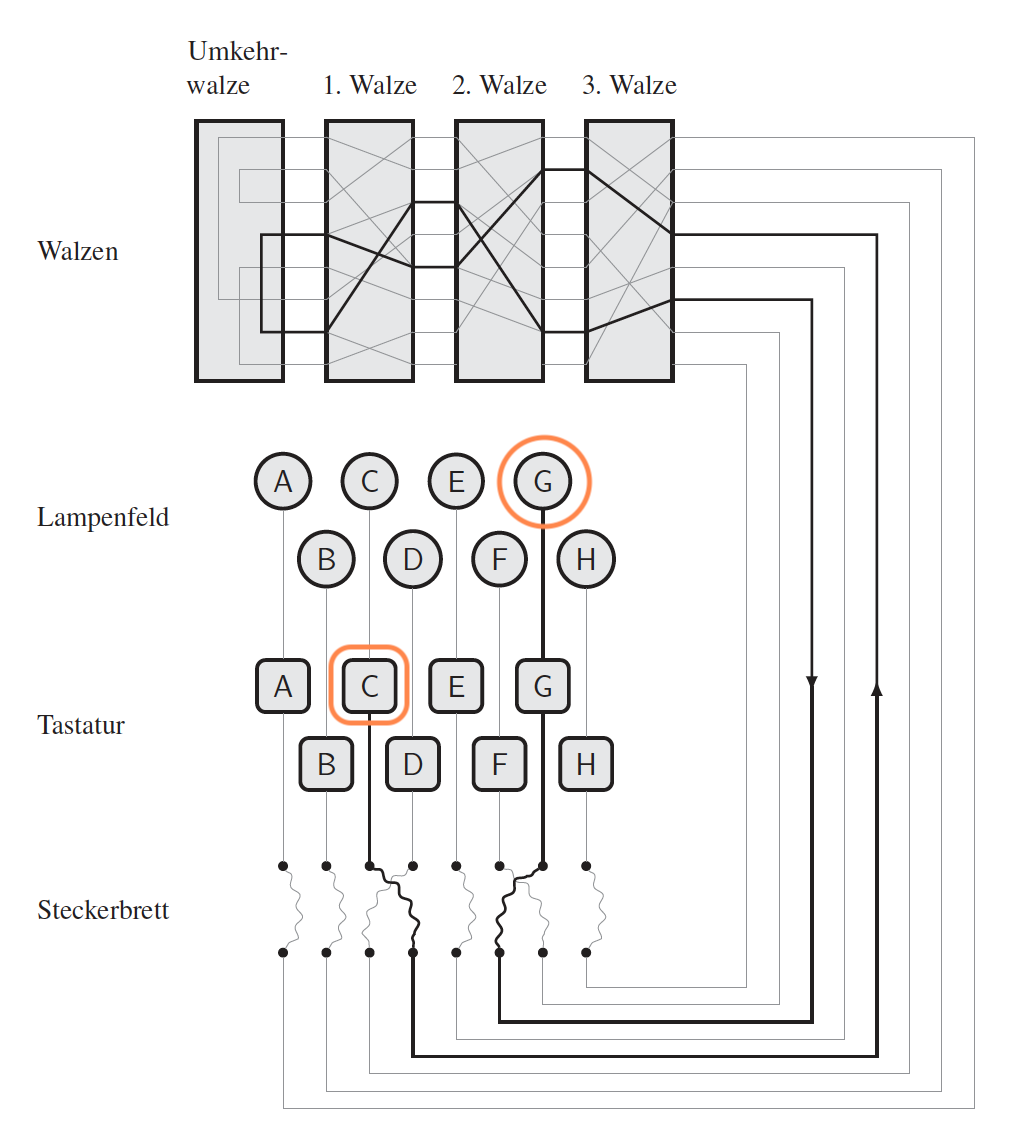
\includegraphics[scale=0.3]{enigma_funktionsweise_vereinfacht.png}
	\caption{Komponenten und die Verdrahtung der \texttt{ENIGMA} \cite{freiermuth2014kryptologie}.}
	\label{figure-enigma-aufbau}
	\end{minipage}
\end{figure}

\vspace{-0.5cm}

\section{Schlüsselmenge}

Die \texttt{ENIGMA} besitzt mindestens\footnote{Das Ergebnis beinhaltet nicht die verschiedenen Ringstellungen der \texttt{ENIGMA}.} \num{158962555217826360000} verschiedene Schlüssel. Das sind also mehr als \num{100} Trillionen ($=10^{20}$) Schlüssel. Dies entspricht einer Schlüssellänge von $log_2(10^{20}) \approx 67$ Bits. Im Vergleich dazu besitzt das symmetrische Kryptosystem \ac{DES} eine Schlüssellänge von $56$ Bits. Es wurde in den 1970er Jahren entwickelt und bis in den 1990er Jahren eingesetzt.

\section{Zusätzliches Videomaterial}

Das erste Video zeigt die Idee der Kryptoanalyse.

\begin{itemize}
	\item Flaw in the Enigma Code: \url{https://youtu.be/V4V2bpZlqx8}
	\item Turing's Enigma Problem (Part 1): \url{https://youtu.be/d2NWPG2gB_A}
	\item Turing's Enigma Problem (Part 2): \url{https://youtu.be/kj_7Jc1mS9k}
	\item Cracking Enigma in 2021: \url{https://youtu.be/RzWB5jL5RX0}
	\item How did the Enigma Machine work? \url{https://youtu.be/ybkkiGtJmkM}
\end{itemize}

\section{Aufgaben}

\begin{enumerate}
\item Ist die \texttt{ENIGMA} ein polyalphabetisches Kryptosystem? Begründen Sie Ihre Antwort.

\fillwithgrid{\stretch{1}}

\newpage

\item Aus welchen Teilen besteht der Schlüssel bei der \texttt{ENIGMA}? Recherchieren und erklären Sie den Schlüsselaufbau. Nennen Sie dann einen konkreten Schlüssel als Beispiel.

\fillwithgrid{2in}

\item Warum ist die \texttt{ENIGMA} ein symmetrisches Kryptosystem? Erklären Sie detailliert.

\fillwithgrid{1in}

\item Die \texttt{ENIGMA} ist so konstruiert, dass ein Klartextbuchstabe niemals zum gleichen Kryptotextbuchstabe verschlüsselt wird. Beispiel: Der Klartextbuchstabe K wird niemals zum Kryptotextbuchstabe K verschlüsselt. Nehmen Sie zu dieser Konstruktionsentscheidung hinsichtlich der Sicherheit der \texttt{ENIGMA} Stellung.

\fillwithgrid{1in}

\item Verschlüsseln Sie den Klartext TURING mit dem Emulator (\url{https://www.101computing.net/enigma-machine-emulator}). Verwenden Sie folgenden Schlüssel:
\begin{itemize}
\item Reflector (Umkehrwalze): UKW-B
\item Rotor (Walzenlage): \textrm{III}, \textrm{I}, \textrm{V}
\item Ring Setting (Ringstellung): A, A, A
\item Initial Position (Grundstellung): F, O, O
\item Plugboard (Steckerbrett): K $\rightarrow$ S, W $\rightarrow$ E, G $\rightarrow$ Y, F $\rightarrow$ M
\end{itemize}

\fillwithgrid{0.25in}

% CWVDHJ

\item Entschlüsseln Sie den Kryptotext TXWXOXKRI mit dem Emulator (\url{https://www.101computing.net/enigma-machine-emulator}). Verwenden Sie folgenden Schlüssel:
\begin{itemize}
\item Reflector (Umkehrwalze): UKW-B
\item Rotor (Walzenlage): \textrm{IV}, \textrm{II}, \textrm{III}
\item Ring Setting (Ringstellung): A, A, A
\item Initial Position (Grundstellung): M, I, X
\item Plugboard (Steckerbrett): A $\rightarrow$ D, C $\rightarrow$ N, E $\rightarrow$ T, F $\rightarrow$ L, H $\rightarrow$ I, J $\rightarrow$ V
\end{itemize}

% SCHERBIUS

\fillwithgrid{0.25in}

\end{enumerate}
